\chapter{A-A WEAPONS}
\thumbtab{A-A}{5}
\localtableofcontents
\cleardoublepage

\section{AIR-TO-AIR GUNNERY}

\subsection{M-61 VULCAN}
\label{subsec:m61}

\begin{tcoloritemize}
    \blueitem{M-61 Vulcan}{
    Internally mounted, high fire-rate, 20mm rotary ``Gattling'' cannon.
    In service since 1959

    \begin{subitemize}
        \item \textbf{Fire Rate} --- 6000rpm
        \item \textbf{Round Size} --- 20mm
        \item \textbf{Ammo Capacity} --- 510 rounds
    \end{subitemize}}
\end{tcoloritemize}

\begin{figure}[htbp]
    \centering
    \fbox{
    \begin{minipage}[t][40mm][t]{100mm}
        \center{\large\textbf{M-61 OVERVIEW}}
        \begin{itemize}
            \item Some kind of overview figure
            \item maybe showing side on profile of the weapon?
        \end{itemize}
    \end{minipage}
    }
    \caption{M-61 Vulcan}
\end{figure}
    
\begin{tcoloritemize}
    \blueitem{Ammunition Types}{
    \begin{subitemize}
        \item \textbf{HEI} --- \textbf{H}igh \textbf{E}xplosive \textbf{I}ncendiary
        \item \textbf{HEI-T} --- \textbf{H}igh \textbf{E}xplosive \textbf{I}ncendiary-\textbf{T}racer
        \item \textbf{AP} --- \textbf{A}rmor \textbf{P}iercing
        \item \textbf{TP} --- \textbf{T}arget \textbf{P}ractice
        \item \textbf{SAPHEI} --- \textbf{S}emi \textbf{A}rmor \textbf{P}iercing \textbf{H}igh \textbf{E}xplosive \textbf{I}ncendiary
    \end{subitemize}}
    \blueitem{Gunsight / \break Cueing Modes}{
    \begin{subitemize}
        \item \textbf{EEGS} --- \textbf{E}nhanced \textbf{E}nvelope \textbf{G}un\textbf{S}ight \\
        \hyperref[subsec:m61:eegssymb]{See \Cref{subsec:m61:eegssymb}}
        \item \textbf{Employment w/o radar track (EEGS level II)} \\
        \hyperref[subsec:m61:eegslvl2]{See \Cref{subsec:m61:eegslvl2}}
        \item \textbf{Employment with radar track (EEGS level V)} \\
        \hyperref[subsec:m61:eegslvl5]{See \Cref{subsec:m61:eegslvl5}}
    \end{subitemize}}
    \blueitem{Select GUN}{
    Via Dogfight --- AIM-9 \& GUN automatically selected

    \begin{subenumerate}
        \item \textbf{DGFT/MSL OVRD} \dotfill \textbf{DGFT}
    \end{subenumerate}

    Via A-A Master Mode

    \begin{subenumerate}
        \item \textbf{Master Mode} \dotfill \textbf{A-A}
        \item \textbf{SMS OSB 1} \dotfill \textbf{Cycle to GUN}
    \end{subenumerate}}
\end{tcoloritemize}

\subsubsection{SMS CONTROLS}
\label{subsec:m61:sms}
\begin{tcoloritemize}
    \blueitem{Operating Mode}{\textbf{OSB 1} cycles A-A modes, should display \textbf{GUN}}
    \blueitem{Sub-Mode}{\textbf{OSB 2} cycles gunsight modes
    
    \begin{subitemize}
        \item \textbf{EEGS} --- \textbf{E}nhanced \textbf{E}nvelope \textbf{G}un\textbf{S}ight \\
        \textbf{See \Cref{subsec:m61:eegssymb}}
    \end{subitemize}}
    \blueitem{Rounds \break Remaining}{Indicates number of rounds remaining in 10s}
\end{tcoloritemize}

\begin{figure}[htbp]
    \centering
    \begin{tikzpicture}[auto, node distance=10mm, x=1mm, y=1mm, very thick, line cap=round,
        >={Latex[round]}
        ]
        
        \node[] (fig) at (0,0) {
            \includegraphics[
                height=75mm,
                page={79},
            ]{F16_aaweapons_v10_NoBackgroundImages.pdf}
        };

        \node[] at (0,0) {\color{red}\textbf{MISSING ANNOTATIONS}};
    \end{tikzpicture}
    % \fbox{
    % \begin{minipage}[t][75mm][t]{100mm}
    %     \center{\large\textbf{MFD --- SMS --- GUN CONTROLS}}
    %     \begin{itemize}
    %         \item show sms gun page
    %         \item label each of the relevant controls explained in text
    %     \end{itemize}
    % \end{minipage}
    % }
    \caption{MFD SMS Gun Controls}
\end{figure}

\subsubsection{EEGS SYMBOLOGY}
\label{subsec:m61:eegssymb}
\begin{tcoloritemize}
    \blueitem{EEGS}{\textbf{E}nhanced \textbf{E}nvelope \textbf{G}un\textbf{S}ight

    \begin{subitemize}
        \item \textbf{Provides multiple levels of symbology depending on presence of radar lock}
    \end{subitemize}}
    \blueitem{Level I}{Backup mode displaying only boresight cross in event of INS failure}
    \blueitem{Level II}{Operating mode prior to radar lock

    \begin{subitemize}
        \item \textbf{Boresight Cross} --- shows where gun / aircraft is pointed
        \item \textbf{EEGS Funnel}
        \begin{itemize}
            \item displays path of rounds through space
            \item funnel is of set width to judge distance --- adjust width to target wingspan, stabilize edges of funnel on wingtips and fire
        \end{itemize}
        \item \textbf{MGRS} --- \textbf{M}ultiple \textbf{R}eference \textbf{G}un\textbf{S}ight
        \begin{itemize}
            \item 5 line-segments pointing towards boresight
            \item reference for high aspect snap shots (placeing target on MGRS line should have it fly through gun cross)
        \end{itemize}
    \end{subitemize}
    
    Reference symbology in \cref{fig:aaweap:m61:eegslvl2} and \cref{fig:aaweap:m61:eegsfunnel}
    }
    \blueitem{Level III / IV}{Intermediate modes during radar lock acquisition}
    \blueitem{Level V}{Operating mode with radar lock. Level II symbology is retained with additional elements
    
    \begin{subitemize}
        \item \textbf{Level V Pipper}
        \begin{itemize}
            \item gunfire solution --- stabilize pipper on target and fire
            \item contains additional range/aspect cues
        \end{itemize}
        \item \textbf{Range Caret}
        \begin{itemize}
            \item displayed on \underline{inside} edge of level V pipper
            \item unwinds from 12 o'clock at 12'000ft counter-clockwise
        \end{itemize}
        \item \textbf{Aspect Caret} 
        \begin{itemize}
            \item displayed on \underline{outside} edge of level V pipper
        \end{itemize}
        \item \textbf{T-Symbol}
        \begin{itemize}
            \item \textbf{``--- + ---'' 1G Pipper} --- lead angle for non-maneuvering target,
            flanking horizontal lines indicate out-of-plane maneuver potential of target
            \item \textbf{``---'' Max-G Pipper} --- lead angle for target pulling max-G towards you
        \end{itemize}
        \item \textbf{BATR} --- \textbf{B}ullets \textbf{A}t \textbf{T}arget \textbf{R}ange
        \begin{itemize}
            \item displayed once rounds have been fired
            \item dissappears after last round has passed beyond target range
            \item useful to evaluate shots (also for training)
        \end{itemize}
    \end{subitemize}
    
    Reference symbology in \cref{fig:aaweap:m61:eegslvl5} and \cref{fig:aaweap:m61:eegspipper}
    }
\end{tcoloritemize}

\begin{figure}[htbp]
    \centering

    \begin{tikzpicture}[auto, node distance=10mm, x=1mm, y=1mm, very thick, line cap=round,
        >={Latex[round]}
        ]
        
        \node[draw, rounded corners] (fig) at (0,0) {
            \includegraphics[
                height=75mm,
                page={80},
            ]{F16_aaweapons_v10_NoBackgroundImages.pdf}
        };

        \node[] at (0,0) {\color{red}\textbf{MISSING ANNOTATIONS}};
    \end{tikzpicture}
    % \fbox{
    % \begin{minipage}[t][75mm][t]{100mm}
    %     \center{\large\textbf{HUD --- EEGS LVL II}}
    %     \begin{itemize}
    %         \item show EEGS LVL II symbology of the HUD
    %         \item maybe with a simiplified target outline ``mid pull'' in the funnel?
    %         \begin{itemize}
    %             \item if don't have target here maybe put in marginfig below? (just show funnel with target at correct point to shoot)
    %             \item alternatively, maybe have separate figure just showing target in funnel here? (could be reused as marginfig below)
    %         \end{itemize}
    %     \end{itemize}
    % \end{minipage}
    % }
    \caption{EEGS LVL II HUD Symbology}
    \label{fig:aaweap:m61:eegslvl2}
\end{figure}

\begin{figure}[htbp]
    \centering

    \begin{tikzpicture}[auto, node distance=10mm, x=1mm, y=1mm, very thick, line cap=round,
        >={Latex[round]}
        ]
        
        \node[draw, rounded corners] (fig) at (0,0) {
            \includegraphics[
                height=75mm,
                page={84},
            ]{F16_aaweapons_v10_NoBackgroundImages.pdf}
        };

        \node[] at (0,0) {\color{red}\textbf{MISSING ANNOTATIONS}};
    \end{tikzpicture}
    % \fbox{
    % \begin{minipage}[t][75mm][t]{100mm}
    %     \center{\large\textbf{HUD --- EEGS LVL V}}
    %     \begin{itemize}
    %         \item show EEGS LVL V symbology of the HUD
    %         \item maybe with a simiplified target outline ``mid pull'' in the funnel?
    %         \begin{itemize}
    %             \item more necessary here since lvl V relies on having a lock
    %             \item maybe have separate figure just showing lvl 5 target pipper since there is a lot going on (could be reuses as marginfig below)
    %         \end{itemize}
    %     \end{itemize}
    % \end{minipage}
    % }
    \caption{EEGS LVL V HUD Symbology}
    \label{fig:aaweap:m61:eegslvl5}
\end{figure}

\begin{figure}[htbp]
    \centering
    \begin{tikzpicture}[auto, node distance=10mm, x=1mm, y=1mm, very thick, line cap=round,
        >={Latex[round]}
        ]
        
        \node[minimum width=\linewidth] (blanker) at (0,0) {};
        \node[draw, rounded corners] (fig) at (0,0) {
            \includegraphics[
                scale=1.25,
                page={2},
            ]{F16_aaweapons_v10_4Items.pdf}
        };

        \node[color2, anchor=west, align=left, font=\small\bfseries] (funnel) at (20,10) {EEGS GUN \\ FUNNEL};
        \node[color2, anchor=west, align=left, font=\small\bfseries] (brst) at (20,32.5) {BORESIGHT \\ CROSS};
        \node[color2, anchor=west, align=left, font=\small\bfseries] (mgrs) at (20,-20) {MGRS \\ LINES};

        \draw[->, color2]
        (funnel.west) -- ++(-12.5,0);
        \draw[->, color2]
        (brst.west) -- ++(-15,0);
        \draw[->, color2]
        (mgrs.west) -- ++(-15,0) -- +(-2.5,-5);
    \end{tikzpicture}
    % \fbox{
    % \begin{minipage}[t][50mm][t]{100mm}
    %     \center{\large\textbf{EEGS Funnel \& LVL V Pipper}}
    %     \begin{itemize}
    %         \item show both funnel and pipper as subfigs
    %         \item include target outline in firing position
    %         \item clearly mark level 5 pipper symbology elements
    %         \begin{itemize}
    %             \item batr
    %             \item range cue
    %             \item aspect
    %         \end{itemize}
    %     \end{itemize}
    % \end{minipage}
    % }
    \caption{EEGS Funnel}
    \label{fig:aaweap:m61:eegsfunnel}
\end{figure}

\begin{figure}[htbp]
    \centering
    \begin{tikzpicture}[auto, node distance=10mm, x=1mm, y=1mm, very thick, line cap=round,
        >={Latex[round]}
        ]

        \node[draw, rounded corners] (pipper) at (0,0) {
            \includegraphics[
                scale=1.25,
                page={99},
            ]{F16_aaweapons_v11.pdf}
        };
        \node[
            anchor=north,
            align=center,
            font=\small\bfseries
        ](mark1)at(pipper.south){EEGS LVL 5 PIPPER};

        \node[draw, rounded corners, left=10mm of pipper] (tsymb) {
            \includegraphics[
                scale=1.25,
                page={101},
            ]{F16_aaweapons_v11.pdf}
        };
        \node[
            anchor=north,
            align=center,
            font=\small\bfseries
        ](mark2)at(tsymb.south){T-SYMBOL};

        \node[draw, rounded corners, left=10mm of tsymb] (tdes) {
            \includegraphics[
                scale=1.25,
                page={100},
            ]{F16_aaweapons_v10_NoBackgroundImages.pdf}
        };
        \node[
            anchor=north,
            align=center,
            font=\small\bfseries
        ](mark3)at(tdes.south){TARGET DESIGNATOR};

        \path[] (tdes) -- node[pos=0.5, anchor=center]{\textbf{+}}(tsymb);
        \path[] (tsymb) -- node[pos=0.5, anchor=center]{\textbf{=}}(pipper);
    \end{tikzpicture}
    \caption{EEGS Level V Pipper}
    \label{fig:aaweap:m61:eegspipper}
\end{figure}

\marginfigeometry

\subsubsection{GUN SELECTION}
\label{subsec:m61:selection}
\begin{checklistitemize}
    \blueitem{Via Dogfight}{(GUN automatically selected)
    \begin{subenumerate}
        \item \textbf{DGFT/MSL OVRD} \dotfill \textbf{DGFT}
    \end{subenumerate}}
    \blueitem{Via A-A Master Mode}{
    \begin{subenumerate}
        \item \textbf{Master Mode} \dotfill \textbf{A-A}
        \item \textbf{SMS OSB 1} \dotfill \textbf{Cycle to GUN}
    \end{subenumerate}}
    \blueitem{EEGS Symbology}{Verify
    \begin{subitemize}
        \item \textbf{EEGS Level II} appears if no lock present
        \item \textbf{EEGS Level V} appears if target locked
    \end{subitemize}}
\end{checklistitemize}

\subsubsection{EEGS LVL II EMPLOYMENT --- NO RADAR}
\label{subsec:m61:eegslvl2}
\begin{checklistenumerate}
    \blueitem{Prerequisites}{
    \begin{subitemize}
        \item \textbf{RF Switch} \dotfill \textbf{SILENT} \\
        \hfill (if desired, completely silences radar)
        \item \textbf{Selected Weapon} \dotfill \textbf{GUN}
        \item \textbf{Master Arm} \dotfill \textbf{ARM}
    \end{subitemize}}
    \blueitem{Acquire Firing Solution}{
    \marginpar{
        \captionsetup{type=figure}
        \centering
        \begin{tikzpicture}[auto, node distance=10mm, x=1mm, y=1mm, very thick, line cap=round,
            >={Latex[round]}
            ]
            
            \node[draw, rounded corners, minimum width=\marginparwidth] (fig) at (0,0) {
                \includegraphics[
                    scale=1.25,
                    page={2},
                ]{F16_aaweapons_v10_4Items.pdf}
            };
        \end{tikzpicture}
        % \includegraphics[
        %     width=\marginparwidth,
        %     page={2},
        % ]{F16_aaweapons_v10_4Items.pdf}
        % \fbox{
        %     \begin{minipage}[t][40mm][t]{\marginparwidth}
        %         \center{\textbf{EEGS Funnel}}
        %         \begin{itemize}[leftmargin=1em]
        %             \item show funnel on target
        %             \item potentially reuse from above
        %         \end{itemize}
        %     \end{minipage}
        % }
        \caption{EEGS Funnel \& MGRS Lines. Target is approx. aligned with funnel.}
    }

    \smallskip
    Using EEGS funnel

    \begin{subenumerate}
        \item \textbf{EEGS Funnel} \dotfill \textbf{Stabilized On-Target}
        \item \textbf{Funnel Lines} \dotfill \textbf{On target wingtips}
    \end{subenumerate}
    
    % \marginpar{
    %     \captionsetup{type=figure}
    %     \fbox{
    %         \begin{minipage}[t][40mm][t]{\marginparwidth}
    %             \center{\textbf{MGRS Lines}}
    %             \begin{itemize}[leftmargin=1em]
    %                 \item show MGRS line on target
    %                 \item not sure if this fig is necessary
    %                 \item maybe could modify fig from above
    %             \end{itemize}
    %         \end{minipage}
    %     }
    %     \caption{MGRS Lines}
    % }
    Using MGRS lines
    
    \begin{subenumerate}
        \item \textbf{MGRS Line} \dotfill \textbf{Aligned with target}
    \end{subenumerate}}
    \blueitem{Fire Gun}{
    \begin{subenumerate}
        \item \textbf{TRIGGER} \dotfill \textbf{2nd Detent}
        \item Adjust lead to achieve desired effects
    \end{subenumerate}}
\end{checklistenumerate}

\notebox{
    \small
    \textbf{Exact position of target relative to funnel lines dependent on funnel width and target wingspan, 
    see \Cref{subsec:m61:eegsfunneladjust} for funnel adjustment.}
}

\clearpage

\subsubsection{EEGS LVL V EMPLOYMENT --- RADAR}
\label{subsec:m61:eegslvl5}
\begin{checklistenumerate}
    \blueitem{Prerequisites}{
    \begin{subitemize}
        \item \textbf{FCR Switch} \dotfill \textbf{FCR}
        \item \textbf{RF Switch} \dotfill \textbf{NORM}
        \item \textbf{Selected Weapon} \dotfill \textbf{GUN}
        \item \textbf{Master Arm} \dotfill \textbf{ARM}
    \end{subitemize}}
    \blueitem{Radar Acquisition}{ACM selected automatically in \textbf{DGFT} mode, \textbf{see \Cref{subsec:acm}}

    \begin{subenumerate}
        \item \textbf{ACM Submode} \dotfill \textbf{As desired}
        \item Maneuver to place target in radar scan volume
    \end{subenumerate}}
    \blueitem{Acquire Firing Solution}{
    \marginpar{
        \captionsetup{type=figure}
        \centering
        \begin{tikzpicture}[auto, node distance=10mm, x=1mm, y=1mm, very thick, line cap=round,
            >={Latex[round]}
            ]
            \node[draw, rounded corners, minimum width=\marginparwidth] (fig) at (0,0) {
                \includegraphics[
                    scale=1.25,
                    page={88},
                ]{F16_aaweapons_v10_NoBackgroundImages.pdf}
            };
        \end{tikzpicture}
        % \fbox{
        %     \begin{minipage}[t][40mm][t]{\marginparwidth}
        %         \center{\textbf{EEGS Level V Pipper}}
        %         \begin{itemize}[leftmargin=1em]
        %             \item show pipper on target
        %             \item potentially reuse from above
        %         \end{itemize}
        %     \end{minipage}
        % }
        \caption{EEGS Level V Pipper}
    }
    \begin{subenumerate}
        \item \textbf{Pipper} \dotfill \textbf{Stabilized On-Target}
    \end{subenumerate}}
    \blueitem{Fire Gun}{
    \begin{subenumerate}
        \item \textbf{TRIGGER} \dotfill \textbf{2nd Detent}
        \item Adjust lead to achieve desired effects
    \end{subenumerate}}
\end{checklistenumerate}

\subsubsection{ADJUST EEGS FUNNEL WIDTH}
\label{subsec:m61:eegsfunneladjust}
\begin{checklistenumerate}
    \blueitem{Open DED MAN Page}{
    \begin{subenumerate}
        \item \textbf{ICP LIST Button} \dotfill \textbf{Press}
        \item \textbf{DED MAN Page} \dotfill \textbf{Open (5)} 
    \end{subenumerate}}
    \blueitem{Adjust Wingspan}{
    \begin{subenumerate}
        \item \textbf{WSPAN} \dotfill \textbf{Selected}
        \item \textbf{Desired Value} \dotfill Input on ICP, \textbf{ENTR}
        \item \textbf{WSPAN} \dotfill Verify as desired
    \end{subenumerate}}
\end{checklistenumerate}

\marginfigrestore

\section{AIR-TO-AIR MISSILES}

\subsection{AIM-9 SIDEWINDER}
\label{subsec:aim9}
\begin{figure}[htbp]
    \centering
    \fbox{
    \begin{minipage}[t][75mm][t]{100mm}
        \center{\large\textbf{AIM-9 OVERVIEW}}
        \begin{itemize}
            \item Some kind of overview figure
            \item maybe showing side on profile of the weapon?
        \end{itemize}
    \end{minipage}
    }
    \caption{AIM-9 Sidewinder}
\end{figure}

\begin{tcoloritemize}
    \blueitem{AIM-9 \break Sidewinder}{
    Short-range, fire-and-forget ``dogfight'' missile. First entered service in 1956

    \begin{subitemize}
        \item \textbf{Guidance} --- IR-guided (\textbf{Fox 2})
        \item \textbf{Range} --- min: \textasciitilde3000ft, max: \textasciitilde10-20nm
    \end{subitemize}}
    \blueitem{Variants}{
    \begin{subitemize}
        \item \textbf{9M} --- IR-guided, short range, all-aspect
        \item \textbf{9X} --- HOBS (\textbf{H}igh \textbf{O}ff-\textbf{B}ore\textbf{S}ight) capable, thrust-vectored, all-aspect
    \end{subitemize}}
    \blueitem{Acquisition / Cueing Modes}{
    \begin{subitemize}
        \item \textbf{Acquisition with own missile seeker (BORE)} \\
        \hyperref[subsec:aim9:bore]{See \Cref{subsec:aim9:bore}}
        \item \textbf{Seeker cued with HMD LOS (BORE)} \\
        {See \Cref{subsec:aim9:hmcs}}
        \item \textbf{Seeker slaved to radar track LOS (SLAVE)} \\
        \hyperref[subsec:aim9:slave]{See \Cref{subsec:aim9:slave}}
    \end{subitemize}}
    \blueitem{Select AIM-9}{
    Via Dogfight --- AIM-9 \& GUN automatically selected

    \begin{subenumerate}
        \item \textbf{DGFT/MSL OVRD} \dotfill \textbf{DGFT}
        \item \textbf{Selected Weapon (OSB 7)} \dotfill Verify \textbf{9LM / 9X}
    \end{subenumerate}

    Via Missile Override

    \begin{subenumerate}
        \item \textbf{DGFT/MSL OVRD} \dotfill \textbf{OVRD}
        \item \textbf{Selected Weapon (SMS OSB 7)} \dotfill \textbf{9LM / 9X}
    \end{subenumerate}

    Via A-A Master Mode

    \begin{subenumerate}
        \item \textbf{Master Mode} \dotfill \textbf{A-A}
        \item \textbf{Operating Mode (SMS OSB 1)} \dotfill Verify \textbf{AAM}
        \item \textbf{Selected Weapon (SMS OSB 7)} \dotfill \textbf{9LM / 9X}
    \end{subenumerate}
    
    Selected weapon can also be cycled with \textbf{NWS/MSL Step depress (long)}
    }
\end{tcoloritemize}
    
\subsubsection{SMS CONTROLS}

\begin{tcoloritemize}
    \blueitem{SPOT / SCAN}{
    \textbf{OSB 2} controls seeker field of view
    \begin{subitemize}
        \item \textbf{SPOT} --- Narrow, increased detection range
        \item \textbf{SCAN} --- Wide, decreased detection range
    \end{subitemize}}
    \blueitem{Selected Weapon}{
    \textbf{OSB 7} cycles through available A-A weapon types
    
    \medskip
    Selected weapon can also be cycled with \textbf{NWS/MSL Step depress (long)}
    }
    \blueitem{WARM / COOL}{
    \textbf{OSB 8} controls seeker cooling status

    \begin{subitemize}
        \item \textbf{COOL} ---  increases seeker sensitivity, should be set prior to engagement
        \item Set automatically for \textbf{DGFT} \& \textbf{MSL OVRD}
    \end{subitemize}}
    \blueitem{Selected Station}{
    \textbf{OSB 10 / 16} select/cycle available missile pylons
    
    \medskip
    Selected station can also be cycled with \textbf{NWS/MSL Step depress (short)}
    }
    \blueitem{SLAVE / BORE}{
    \textbf{OSB 19} controls seeker line-of-sight

    \begin{subitemize}
        \item \textbf{BORE} --- \hyperref[subsec:aim9:bore]{\textbf{See \Cref{subsec:aim9:bore}}}
        \begin{itemize}
            \item acquisition with own missile seeker
            \item or cued with HMD (if powered)
            \item \textbf{does NOT require FCR}
        \end{itemize}
        \item \textbf{SLAVE} --- \hyperref[subsec:aim9:slave]{\textbf{See \Cref{subsec:aim9:slave}}}
        \begin{itemize}
            \item seeker slaved to radar track LOS
            \item typically via ACM Modes
        \end{itemize}
    \end{subitemize}
    
    Line-of-sight mode can also be cycled with \textbf{Cursor Enable Depress}}
\end{tcoloritemize}

\begin{figure}[htbp]
    \centering
    \begin{tikzpicture}[auto, node distance=10mm, x=1mm, y=1mm, very thick, line cap=round,
        >={Latex[round]}
        ]
        
        \node[] (fig) at (0,0) {
            \includegraphics[
                height=75mm,
                page={91},
            ]{F16_aaweapons_v10_NoBackgroundImages.pdf}
        };

        \node[] at (0,0) {\color{red}\textbf{MISSING ANNOTATIONS}};
    \end{tikzpicture}
    % \fbox{
    % \begin{minipage}[t][75mm][t]{100mm}
    %     \center{\large\textbf{MFD --- SMS --- AIM-9 CONTROLS}}
    %     \begin{itemize}
    %         \item show sms aim-9 page
    %         \item label each of the relevant controls explained in text
    %     \end{itemize}
    % \end{minipage}
    % }
    \caption{MFD SMS AIM-9 Controls}
\end{figure}

\clearpage

\subsubsection{SYMBOLOGY}
\begin{tcoloritemize}
    \blueitem{MFD Symbology}{Reference \Cref{subsec:aim120:symb}}
    \blueitem{HUD/HMD \break Symbology}{
    \begin{subitemize}
        \item \textbf{Missile Diamond} --- AIM-9 seeker line-of-sight
        \begin{itemize}
            \item displayed on HUD \& HMD
            \item marked with \textbf{X} if beyond seeker limits
        \end{itemize}
        \item \textbf{Missile Reticle} --- AIM-9 seeker field-of-view
        \begin{itemize}
            \item displayed on HUD only
            \item size reflects \textbf{SPOT/SCAN} setting 
        \end{itemize}
        \item \textbf{Dynamic Aiming Cross} --- HMD line-of-sight
    \end{subitemize}

    Reference symbology in \cref{fig:aaweap:aim9:hudsymb}

    \begin{subitemize}
        \item \textbf{DLZ} --- \textbf{D}ynamic \textbf{L}aunch \textbf{Z}one
        \begin{itemize}
            \item displays missile/target range information
            \item reference \Cref{subsec:aim120:symb}
        \end{itemize}
    \end{subitemize}
    }
\end{tcoloritemize}

\begin{figure}[htbp]
    \centering
    \begin{tikzpicture}[auto, node distance=10mm, x=1mm, y=1mm, very thick, line cap=round,
        >={Latex[round]}
        ]
        
        \node[draw, rounded corners] (fig) at (0,0) {
            \includegraphics[
                height=75mm,
                page={92},
            ]{F16_aaweapons_v11.pdf}
        };

        \node[] at (0,0) {\color{red}\textbf{MISSING ANNOTATIONS}};
    \end{tikzpicture}
    % \fbox{
    % \begin{minipage}[t][75mm][t]{100mm}
    %     \center{\large\textbf{HUD/HMD --- AIM-9 Symbology}}
    %     \begin{itemize}
    %         \item show hud/hmd with aim-9 in use 
    %         \item clearly indicate missile diamond/reticle and dynamic aiming cross
    %         \item maybe show several versions?
    %         \begin{itemize}
    %             \item 1 with missile reticle from HUD?
    %             \item 1 with missile diamond latchedon aiming cross?
    %             \item 1 with diamond on target?
    %             \item 1 with \textbf{X}?
    %         \end{itemize}
    %         or some subset of those?
    %         \item can reuse these in marginfigs below?
    %     \end{itemize}
    % \end{minipage}
    % }
    \caption{AIM-9 HUD Symbology}
    \label{fig:aaweap:aim9:hudsymb}
\end{figure}

\begin{figure}[htbp]
    \centering
    \begin{tikzpicture}[auto, node distance=10mm, x=1mm, y=1mm, very thick, line cap=round,
        >={Latex[round]}
        ]
        
        \node[draw, rounded corners] (fig) at (0,0) {
            \includegraphics[
                height=50mm,
                page={3},
            ]{F16_aaweapons_missilelaunch_new_v1_1.pdf}
        };

        \node[] at (0,20) {\color{red}\textbf{MISSING ANNOTATIONS}};
    \end{tikzpicture}
    \caption{AIM-9 HMD Symbology}
    \label{fig:aaweap:aim9:hmdsymb}
\end{figure}

\marginfigeometry

\subsubsection{AIM-9 SELECTION}
\begin{checklistitemize}
    \blueitem{Via DGFT}{(AIM-9 selected automatically)
    \begin{subenumerate}
        \item \textbf{DGFT/MSL OVRD} \dotfill \textbf{DGFT}
    \end{subenumerate}}
    \blueitem{Via MSL OVRD}{
    \begin{subenumerate}
        \item \textbf{DGFT/MSL OVRD} \dotfill \textbf{MSL OVRD}
        \item \textbf{Selected Weapon} \dotfill \textbf{9M/9X}
        \begin{itemize}
            \item \textbf{SMS OSB 7} --- \textbf{Press}
            \item or \textbf{NWS/MSL STEP} --- \textbf{Press (long)}
        \end{itemize}
    \end{subenumerate}}
    \blueitem{Via A-A Master Mode}{
    \begin{subenumerate}
        \item \textbf{Master Mode} \dotfill \textbf{A-A}
        \item \textbf{SMS OSB 1} \dotfill \textbf{Verify AAM} (default)
        \item \textbf{Selected Weapon} \dotfill \textbf{9M/9X}
        \begin{itemize}
            \item \textbf{SMS OSB 7} --- \textbf{Press}
            \item or \textbf{NWS/MSL STEP} --- \textbf{Press (long)}
        \end{itemize}
    \end{subenumerate}}
\end{checklistitemize}

\subsubsection{BORE EMPLOYMENT --- NO RADAR}
\label{subsec:aim9:bore}
\begin{checklistenumerate}
    \blueitem{Prerequisites}{
    \begin{subitemize}
        \item \textbf{RF Switch} \dotfill \textbf{SILENT} \\
        \hfill (if desired, completely silences radar)
        \item \textbf{Selected Weapon} \dotfill \textbf{9M/9X}
        \item \textbf{SLAVE/BORE} \dotfill \textbf{BORE}
        \item \textbf{WARM/COOL} \dotfill Verify \textbf{COOL}
        \item \textbf{Master Arm} \dotfill \textbf{ARM}
    \end{subitemize}}
    \blueitem{AIM-9 Track Acquisition}{
    \marginpar{
        \captionsetup{type=figure}
        \centering
        \begin{tikzpicture}[auto, node distance=10mm, x=1mm, y=1mm, very thick, line cap=round,
            >={Latex[round]}
            ]
            \node[draw, rounded corners, minimum width=\marginparwidth] (fig) at (0,0) {
                \includegraphics[
                    scale=1.25,
                    page={105},
                ]{F16_aaweapons_v11.pdf}
            };
        \end{tikzpicture}
        % \fbox{
        %     \begin{minipage}[t][40mm][t]{\marginparwidth}
        %         \center{\textbf{AIM-9 Track}}
        %         \begin{itemize}[leftmargin=1em]
        %             \item show missile reticle
        %             \item show diamond latched to symbolic target (outline)
        %         \end{itemize}
        %     \end{minipage}
        % }
        \caption{AIM-9 missile diamond latched to target, indicating lock.}
    }
    \begin{subenumerate}
        \item \textbf{Missile Reticle} \dotfill \textbf{On-Target}
        \item \textbf{Sidewinder Audio} \dotfill \textbf{Lock Tone}
        \item \textbf{CAGE/UNCAGE} \dotfill \textbf{Press}
        \item \textbf{Missile Diamond} \dotfill verify latched to target
    \end{subenumerate}}
    \blueitem{Fire Missile}{
    \begin{subenumerate}
        \item Maneuver into firing position
        \item \textbf{Sidewinder Audio} \dotfill \textbf{Lock Tone}
        \item \textbf{WPN REL} \dotfill \textbf{Depress}
    \end{subenumerate}}
\end{checklistenumerate}

\clearpage

\subsubsection{HMCS BORE EMPLOYMENT --- NO RADAR}
\label{subsec:aim9:hmcs}
\begin{checklistenumerate}
    \blueitem{Prerequisites}{
    \begin{subitemize}
        \item \textbf{HMD SYMB. INT} \dotfill \textbf{INT}
        \item \textbf{RF Switch} \dotfill \textbf{SILENT} \\
        \hfill (if desired, completely silences radar)
        \item \textbf{Selected Weapon} \dotfill \textbf{9M/9X}
        \item \textbf{SLAVE/BORE} \dotfill \textbf{BORE}
        \item \textbf{WARM/COOL} \dotfill Verify \textbf{COOL}
        \item \textbf{Master Arm} \dotfill \textbf{ARM}
    \end{subitemize}}
    \blueitem{AIM-9 Track Acquisition}{
    \marginpar{
        \captionsetup{type=figure}
        \begin{tikzpicture}[auto, node distance=10mm, x=1mm, y=1mm, very thick, line cap=round,
            >={Latex[round]}
            ]
            \node[draw, rounded corners, minimum width=\marginparwidth] (fig) at (0,0) {
                \includegraphics[
                    scale=0.75,
                    page={5},
                ]{F16_aaweapons_missilelaunch_new_v1_1.pdf}
            };

            \node[] at (0,0) {\color{red}\textbf{USES RADAR}};
        \end{tikzpicture}
        % \fbox{
        %     \begin{minipage}[t][40mm][t]{\marginparwidth}
        %         \center{\textbf{AIM-9 HMD Track}}
        %         \begin{itemize}[leftmargin=1em]
        %             \item show missile diamond \& dynamic aiming cross
        %             \item show diamond latched to symbolic target?
        %         \end{itemize}
        %     \end{minipage}
        % }
        \caption{AIM-9 HMD Track}
    }
    \marginpar{
        \captionsetup{type=figure}
        \begin{tikzpicture}[auto, node distance=10mm, x=1mm, y=1mm, very thick, line cap=round,
            >={Latex[round]}
            ]
            \node[draw, rounded corners, minimum width=\marginparwidth] (fig) at (0,0) {
                \includegraphics[
                    scale=0.75,
                    page={6},
                ]{F16_aaweapons_missilelaunch_new_v1_1.pdf}
            };
        \end{tikzpicture}
        % \fbox{
        %     \begin{minipage}[t][40mm][t]{\marginparwidth}
        %         \center{\textbf{AIM-9 HMD LOS}}
        %         \begin{itemize}[leftmargin=1em]
        %             \item show missile diamond out of HMD limits
        %             \item can probably reuse from above
        %         \end{itemize}
        %     \end{minipage}
        % }
        \caption{X indicates HMD beyond AIM-9 seeker limits}
    }
    \begin{subenumerate}
        \item Maneuver to place target within AIM-9 seeker limits
        \item \textbf{HMD Aiming Cross} \dotfill \textbf{On-Target}
    \end{subenumerate}

    Missile diamond follows aiming cross (within seeker limits)

    \begin{subenumerate}[start=3]
        \item \textbf{Sidewinder Audio} \dotfill \textbf{Lock Tone}
        \item \textbf{CAGE/UNCAGE} \dotfill \textbf{Press}
        \item \textbf{Missile Diamond} \dotfill verify latched to target
    \end{subenumerate}}
    \blueitem{Fire Missile}{
    \begin{subenumerate}
        \item Maneuver into firing position
        \item \textbf{Sidewinder Audio} \dotfill \textbf{Lock Tone}
        \item \textbf{WPN REL} \dotfill \textbf{Depress}
    \end{subenumerate}}
\end{checklistenumerate}

\begin{figure}[htbp]
    \centering
    \fbox{
    \begin{minipage}[t][40mm][t]{75mm}
        \center{\large\textbf{AIM-9 Envelope}}
        \begin{itemize}
            \item show overhead missile envelope around symbolic target?
            \item this is really a stretch goal \dots
        \end{itemize}
    \end{minipage}
    }
    \caption{AIM-9 Firing envelope}
    \label{fig:aaweap:aim9:envelope}
\end{figure}

\clearpage

\subsubsection{SLAVE EMPLOYMENT --- RADAR}
\label{subsec:aim9:slave}
\begin{checklistenumerate}
    \blueitem{Prerequisites}{
    \begin{subitemize}
        \item \textbf{FCR Switch} \dotfill \textbf{FCR}
        \item \textbf{RF Switch} \dotfill \textbf{NORM}
        \item \textbf{HMD SYMB. INT} \dotfill As desired
        \item \textbf{Selected Weapon} \dotfill \textbf{9M/9X}
        \item \textbf{SLAVE/BORE} \dotfill Verify \textbf{SLAVE}
        \item \textbf{WARM/COOL} \dotfill Verify \textbf{COOL}
        \item \textbf{Master Arm} \dotfill \textbf{ARM}
    \end{subitemize}}
    \blueitem{Radar Acquisition}{ACM selected automatically in \textbf{DGFT} mode, \textbf{see \Cref{subsec:acm}}
    \marginpar{
        \captionsetup{type=figure}
        \centering
        \begin{tikzpicture}[auto, node distance=10mm, x=1mm, y=1mm, very thick, line cap=round,
            >={Latex[round]}
            ]

            \draw[color2, fill=color2!20, dashed] 
            (0,-6) circle [x radius=8, y radius=11.5];
            
            \node[draw, rounded corners, minimum width=\marginparwidth] (bore) at (0,0) {
                \includegraphics[
                    scale=0.5,
                    page={75},
                ]{F16_apg68_RWS_HomePage&SAM_v8.pdf}
            };
        \end{tikzpicture}
        % \fbox{
        %     \begin{minipage}[t][40mm][t]{\marginparwidth}
        %         \center{\textbf{HMD BORE Symbology}}
        %         \begin{itemize}[leftmargin=1em]
        %             \item show HMD BORE circle
        %             \item show symbolic target (outline)
        %             \item can reuse from radar chapter
        %         \end{itemize}
        %     \end{minipage}
        % }
        \caption{HMD BORE scan zone}
    }
    
    \medskip
    For demonstration we will use \textbf{ACM BORE Submode} with HMD
    
    \begin{subenumerate}
        \item \textbf{FCR Mode} \dotfill \textbf{ACM}
        \item \textbf{TMS} \dotfill \textbf{FWD}
        \item \textbf{Target} \dotfill \textbf{In HMD BORE Symbol}
        \item \textbf{Radar} \dotfill wait for \textbf{STT Lock}
    \end{subenumerate}
    
    Can also lock from CRM, \textbf{see \Cref{subsec:crm}}
    }
    \blueitem{AIM-9 Track Acquisition}{
    % \marginpar{
    %     \captionsetup{type=figure}
    %     \centering
    %     \begin{tikzpicture}[auto, node distance=10mm, x=1mm, y=1mm, very thick, line cap=round,
    %         >={Latex[round]}
    %         ]
    %         \node[draw, rounded corners, minimum width=\marginparwidth] (fig) at (0,0) {
    %             \includegraphics[
    %                 scale=1.5,
    %                 page={93},
    %             ]{F16_aaweapons_v11.pdf}
    %         };
    %     \end{tikzpicture}
    %     % \caption{AIM-9 missile diamond latched to target, indicating lock.}
    % }
    \marginpar{
        \captionsetup{type=figure}
        \centering
        \begin{tikzpicture}[auto, node distance=10mm, x=1mm, y=1mm, very thick, line cap=round,
            >={Latex[round]}
            ]
            \node[draw, rounded corners, minimum width=\marginparwidth] (fig) at (0,0) {
                \includegraphics[
                    scale=1.25,
                    page={97},
                ]{F16_aaweapons_v10_NoBackgroundImages.pdf}
            };
        \end{tikzpicture}
        
        % \fbox{
        %     \begin{minipage}[t][40mm][t]{\marginparwidth}
        %         \center{\textbf{AIM-9 Radar Track}}
        %         \begin{itemize}[leftmargin=1em]
        %             \item show radar target designator box
        %             \item show diamond latched to target designator box
        %         \end{itemize}
        %     \end{minipage}
        % }
        \caption{AIM-9 missile diamond and target designator box latched to target, indicating radar and seeker lock.}
    }
    \begin{subenumerate}
        \item \textbf{CAGE/UNCAGE} \dotfill \textbf{Press}
        \item \textbf{Sidewinder Audio} \dotfill \textbf{Lock Tone}
        \item \textbf{Missile Diamond} \dotfill verify latched to target
    \end{subenumerate}}
    \blueitem{Fire Missile}{
    \marginpar{
        \captionsetup{type=figure}
        \centering
        \begin{tikzpicture}[auto, node distance=10mm, x=1mm, y=1mm, very thick, line cap=round,
            >={Latex[round]}
            ]
            \node[draw, rounded corners, minimum width=\marginparwidth] (fig) at (0,0) {
                \includegraphics[
                    scale=2.5,
                    page={104},
                ]{F16_aaweapons_v11.pdf}
            };
        \end{tikzpicture}
        % \fbox{
        %     \begin{minipage}[t][60mm][t]{\marginparwidth}
        %         \center{\textbf{AIM-9 DLZ}}
        %         \begin{itemize}[leftmargin=1em]
        %             \item show DLZ and indicate in-range symbology
        %             \item can probably just reuse from aim-120
        %             \item maybe link to explanation of dlz?
        %         \end{itemize}
        %     \end{minipage}
        % }
        \caption{In-range DLZ}
    }
    \begin{subenumerate}
        \item Maneuver into firing position
        \item \textbf{DLZ} \dotfill indicates \textbf{In-Range}
        \item \textbf{Sidewinder Audio} \dotfill \textbf{Lock Tone}
        \item \textbf{WPN REL} \dotfill \textbf{Depress}
    \end{subenumerate}}
\end{checklistenumerate}

\marginfigrestore 

\subsection{AIM-120 AMRAAM}
\label{subsec:aim120}
\begin{figure}[htbp]
    \centering
    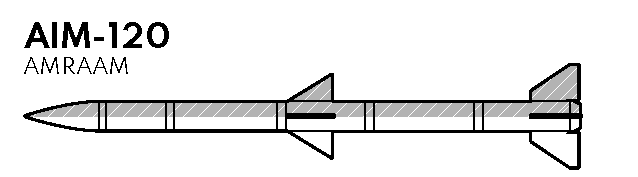
\includegraphics[
            width = 108mm,
    ]{F16_aaweapons_amraam_overview_v01.pdf}
    \fbox{
    \begin{minipage}[t][25mm][t]{100mm}
        \center{\large\textbf{AIM-120 OVERVIEW}}
        \begin{itemize}
            \item Some kind of overview figure
        \end{itemize}
    \end{minipage}
    }
    \caption{AIM-120 AMRAAM}
\end{figure}

\begin{tcoloritemize}
    \blueitem{AIM-120 \break AMRAAM}{
    \textbf{A}dvanced \textbf{M}edium \textbf{R}ange \textbf{A}ir-to-\textbf{A}ir \textbf{M}issile
    --- long range, fire-and-forget, active-radar homing missile

    \begin{subitemize}
        \item \textbf{Guidance} --- Active Radar-Guided (\textbf{Fox 3})
        \item \textbf{Range} --- max:  \textasciitilde30-40nm (high mach, alt)
    \end{subitemize}}
    \blueitem{Employment \break Types}{
    \begin{subitemize}
        \item \textbf{Maddog / Active Launch  (no radar)} \\
        \hyperref[subsec:aim120:maddog]{See \Cref{subsec:aim120:maddog}}
        \item \textbf{Single-target employment (STT lock or TWS/DTT bug)}
        \hyperref[subsec:aim120:single]{See \Cref{subsec:aim120:single}}
        \item \textbf{Multi-target employment (TWS/DTT bug)} \\
        \hyperref[subsec:aim120:multi]{See \Cref{subsec:aim120:multi}}
    \end{subitemize}}
    \blueitem{Flight Profile}{Successful long-range weapon employment necessitates understanding of flight-profile and tactics
    \begin{subitemize}
        \item \textbf{Mid-Course} --- Guided via \underline{datalink}, launching fighter should maintain radar contact with target
        \item \textbf{Terminal Phase} --- Guided via \underline{internal radar}, launching fighter may break away
    \end{subitemize}
    
    \textbf{See \Cref{subsec:bvr} and \Cref{subsec:bvr:tacticalconsideration}}
    }
    \blueitem{Select AIM-120}{
    Via A-A Master Mode

    \begin{subenumerate}
        \item \textbf{Master Mode} \dotfill \textbf{A-A}
        \item \textbf{Operating Mode (SMS OSB 1)} \dotfill Verify \textbf{AAM}
        \item \textbf{Selected Weapon (SMS OSB 7)} \dotfill \textbf{120C}
    \end{subenumerate}

    Via Missile Override

    \begin{subenumerate}
        \item \textbf{DGFT/MSL OVRD} \dotfill \textbf{OVRD}
        \item \textbf{Selected Weapon (SMS OSB 7)} \dotfill \textbf{120C} 
    \end{subenumerate}
    
    Via Dogfight

    \begin{subenumerate}
        \item \textbf{DGFT/MSL OVRD} \dotfill \textbf{DGFT}
        \item \textbf{Selected Weapon (SMS OSB 7)} \dotfill \textbf{120C}
    \end{subenumerate}
    
    Selected weapon can also be cycled with \textbf{NWS/MSL Step depress (long)}
    }
\end{tcoloritemize}

\clearpage

\subsubsection{SMS CONTROLS}
\label{subsec:aim120:sms}
\begin{tcoloritemize}
    \blueitem{Selected Weapon}{
    \textbf{OSB 7} cycles through available A-A weapon types
    
    \medskip
    Selected weapon can also be cycled with \textbf{NWS/MSL Step depress (long)}
    }
    \blueitem{Selected Station}{
    \textbf{OSB 10 / 16} select/cycle availabel missile pylons
    
    \medskip
    Selected station can also be cycled with \textbf{NWS/MSL Step depress (short)}
    }
    \blueitem{SLAVE / BORE}{\textbf{OSB 19} controls missile radar line-of-sight
    \begin{subitemize}
        \item \textbf{SLAVE} --- Missile LOS slaved to AC radar 
        \begin{itemize}
            \item receives DL updates until within own radar limits
        \end{itemize}
        \item \textbf{BORE} --- Missile scans straight ahead
        \begin{itemize}
            \item tracks first detected target
        \end{itemize}
    \end{subitemize}
    
    Line-of-sight mode can also be cycled with \textbf{Cursor Enable Depress}}
\end{tcoloritemize}

\begin{figure}[htbp]
    \centering
    \begin{tikzpicture}[auto, node distance=10mm, x=1mm, y=1mm, very thick, line cap=round,
        >={Latex[round]}
        ]
        
        \node[] (fig) at (0,0) {
            \includegraphics[
                height=75mm,
                page={7},
            ]{F16_aaweapons_missilelaunch_new_v1_1.pdf}
        };

        \node[] at (0,0) {\color{red}\textbf{MISSING ANNOTATIONS}};
    \end{tikzpicture}
    % \fbox{
    % \begin{minipage}[t][75mm][t]{100mm}
    %     \center{\large\textbf{MFD --- SMS --- AIM-120 CONTROLS}}
    %     \begin{itemize}
    %         \item show sms aim-120 page
    %         \item label each of the relevant controls explained in text
    %     \end{itemize}
    % \end{minipage}
    % }
    \caption{MFD SMS AIM-120 Controls}
\end{figure}

\clearpage

\subsubsection{SYMBOLOGY}
\label{subsec:aim120:symb}

\begin{tcoloritemize}
    \blueitem{Basic Radar Symbology}{For beyond-visual-range radar usage and symbology \textbf{reference \Crefrange{subsec:crm}{subsec:tws}}}
    \blueitem{DLZ}{\textbf{D}ynamic \textbf{L}aunch \textbf{Z}one
    \begin{subitemize}
        \item \textbf{Displays target range \& missile performance information on HUD \& FCR Page with}
        \begin{itemize}
            \item missile selected
            \item radar track acquired
        \end{itemize}
        \item \textbf{R\textsubscript{aero} --- Aerodynamic range}
        \begin{itemize}
            \item \underline{maximum kinetic range}
            \item assumes non-maneuvering target
        \end{itemize}
        \item \textbf{R\textsubscript{TR} --- Turn-and-run range}
        \begin{itemize}
            \item maximum range assuming target turns cold at current velocity
        \end{itemize}
        \item \textbf{R\textsubscript{ACT} --- Active range}
        \begin{itemize}
            \item range at which AIM-120 will go active
        \end{itemize}
        \item \textbf{R\textsubscript{MIN} --- Minimum range}
        \item \textbf{Countdown}
        \begin{itemize}
            \item \textbf{A} --- seconds until missile goes active
            \item \textbf{T} --- seconds until predicted impact
        \end{itemize}
    \end{subitemize}}
    \blueitem{ASC \& ASEC}{
    \begin{subitemize}
        \item \textbf{Displays target lead cues to maximize missile performance on HUD \& FCR Page with}
        \begin{itemize}
            \item AIM-120 selected
            \item radar track acquired
        \end{itemize}
        \item \textbf{Pilot should place ASC inside ASEC}
        \item \textbf{ASC} --- \textbf{A}ttack \textbf{S}teering \textbf{C}ue
        \item \textbf{ASEC} --- \textbf{A}llowable \textbf{S}teering \textbf{E}rror \textbf{C}ircle
        \begin{itemize}
            \item dynamically adjusts size based on target maneuvers
            \item fixed size prior to target designation
        \end{itemize}
    \end{subitemize}}
\end{tcoloritemize}

\clearpage

\begin{figure}[htbp]
    \centering
    \begin{subfigure}[b]{0.3\linewidth}
        \centering
        \begin{tikzpicture}[auto, node distance=10mm, x=1mm, y=1mm, very thick, line cap=round,
            >={Latex[round]}
            ]

            \node[draw, rounded corners] (fig) at (0,0) {
                \includegraphics[
                    % height=75mm,
                    scale=0.5,
                    page={16},
                ]{F16_aaweapons_missilelaunch_new_v1_1.pdf}
            };
        \end{tikzpicture}
        \caption{pre-launch}
        \label{fig:aaweap:aim120:dlz:pre}
    \end{subfigure}
    \begin{subfigure}[b]{0.3\linewidth}
        \centering
        \begin{tikzpicture}[auto, node distance=10mm, x=1mm, y=1mm, very thick, line cap=round,
            >={Latex[round]}
            ]

            \node[draw, rounded corners] (fig) at (0,0) {
                \includegraphics[
                    % height=75mm,
                    scale=0.5,
                    page={20},
                ]{F16_aaweapons_missilelaunch_new_v1_1.pdf}
            };



        \node[] at (0,-10) {\color{red}\textbf{MISSING ANNOTATIONS}};
        \end{tikzpicture}
        \caption{post-launch}
        \label{fig:aaweap:aim120:dlz:post}
    \end{subfigure}
    \begin{subfigure}[b]{0.3\linewidth}
        \centering
        \begin{tikzpicture}[auto, node distance=10mm, x=1mm, y=1mm, very thick, line cap=round,
            >={Latex[round]}
            ]

            \node[draw, rounded corners] (fig) at (0,0) {
                \includegraphics[
                    % height=75mm,
                    scale=0.5,
                    page={24},
                ]{F16_aaweapons_missilelaunch_new_v1_1.pdf}
            };
        \end{tikzpicture}
        \caption{post-active}
        \label{fig:aaweap:aim120:dlz:act}
    \end{subfigure}
    % \fbox{
    % \begin{minipage}[t][50mm][t]{100mm}
    %     \center{\large\textbf{DLZ/ASEC/ASC}}
    %     \begin{itemize}
    %         \item show dlz with stuff from text labeled
    %         \item show combined asc/asec symbology
    %     \end{itemize}
    % \end{minipage}
    % }
    \caption{Missile DLZ and Symbology}
\end{figure}

\begin{figure}[htbp]
    \centering
    \begin{tikzpicture}[auto, node distance=10mm, x=1mm, y=1mm, very thick, line cap=round,
        >={Latex[round]}
        ]

        \node[draw, rounded corners] (fig) at (0,0) {
            \includegraphics[
                % height=75mm,
                scale=0.5,
                page={15},
            ]{F16_aaweapons_missilelaunch_new_v1_1.pdf}
        };

        \node[] at (30,0) {\color{red}\textbf{NOT FINISHED}};
    \end{tikzpicture}
    % \fbox{
    % \begin{minipage}[t][50mm][t]{100mm}
    %     \center{\large\textbf{DLZ/ASEC/ASC}}
    %     \begin{itemize}
    %         \item show dlz with stuff from text labeled
    %         \item show combined asc/asec symbology
    %     \end{itemize}
    % \end{minipage}
    % }
    \caption{Missile ASC/ASEC Symbology}
\end{figure}

\begin{tcoloritemize}
    \blueitem{Designator Box}{Box around target when within HUD view}
    \blueitem{TLL}{\textbf{T}arget \textbf{L}ocator \textbf{L}ine
    
    \begin{subitemize}
        \item \textbf{Extends from boresight cross towards target}
        \item \textbf{Relative angle displayed next to boresight cross}
        \item \textbf{Displayed when target is not within HUD field-of-view}
    \end{subitemize}}
    \blueitem{Missile Diamond}{Indicates missile seeker line-of-sight}
    \blueitem{Post-Launch Symbology}{Bugged track symbology is modified to reflect missile launch \& status

    \begin{subitemize}
        \item \textbf{Post-launch} --- Thick ``tail'' is added
        \item \textbf{Post-active} --- Tail begins to flash
        \item \textbf{Post predicted impact} --- Red cross flashes over track
    \end{subitemize}}
\end{tcoloritemize}

\begin{figure}[htbp]
    \centering
    \begin{tikzpicture}[auto, node distance=10mm, x=1mm, y=1mm, very thick, line cap=round,
        >={Latex[round]}
        ]
        \node[draw, rounded corners] (fig) at (0,0) {
            \includegraphics[
                height=75mm,
                page={11},
            ]{F16_aaweapons_missilelaunch_new_v1_1.pdf}
        };

        \node[] at (0,0) {\color{red}\textbf{MISSING ANNOTATIONS}};
    \end{tikzpicture}
    % \fbox{
    % \begin{minipage}[t][75mm][t]{100mm}
    %     \center{\large\textbf{HUD --- AIM-120 Symbology}}
    %     \begin{itemize}
    %         \item show hud in a-a mode, aim-120 selected
    %         \item label each of the relevant symbology elements explained in text
    %         \item probably makes sense to have one big figure with all the elements in it just to show what the hud looks like
    %         \item label additional stuff not mentioned in text
    %         \begin{itemize}
    %             \item range/bearing information etc.
    %         \end{itemize}
    %     \end{itemize}
    % \end{minipage}
    % }
    \caption{A-A AIM-120 HUD (post-launch)}
\end{figure}

\begin{figure}[htbp]
    \centering
    \begin{tikzpicture}[auto, node distance=10mm, x=1mm, y=1mm, very thick, line cap=round,
        >={Latex[round]}
        ]
        
        \node[] (fig) at (0,0) {
            \includegraphics[
                height=75mm,
                page={17},
            ]{F16_aaweapons_missilelaunch_new_v1_1.pdf}
        };

        \node[] at (0,0) {\color{red}\textbf{MISSING ANNOTATIONS}};
    \end{tikzpicture}
    \caption{A-A AIM-120 FCR post-launch. Note the ``tail'' on the track.}
\end{figure}

\begin{figure}[htbp]
    \centering
    \begin{subfigure}[b]{0.15\linewidth}
        \centering
        \includegraphics[
            scale=0.75,
            page={29},
        ]{F16_aaweapons_missilelaunch_new_v1_1.pdf}
        \caption{Search}
    \end{subfigure}
    \begin{subfigure}[b]{0.15\linewidth}
        \centering
        \includegraphics[
            scale=0.75,
            page={30},
        ]{F16_aaweapons_missilelaunch_new_v1_1.pdf}
        \caption{Track}
    \end{subfigure}
    \begin{subfigure}[b]{0.15\linewidth}
        \centering
        \includegraphics[
            scale=0.75,
            page={31},
        ]{F16_aaweapons_missilelaunch_new_v1_1.pdf}
        \caption{System}
    \end{subfigure}
    \begin{subfigure}[b]{0.15\linewidth}
        \centering
        \includegraphics[
            scale=0.75,
            page={32},
        ]{F16_aaweapons_missilelaunch_new_v1_1.pdf}
        \caption{Cursor}
    \end{subfigure}
    \begin{subfigure}[b]{0.15\linewidth}
        \centering
        \includegraphics[
            scale=0.75,
            page={33},
        ]{F16_aaweapons_missilelaunch_new_v1_1.pdf}
        \caption{Bugged}
    \end{subfigure}
    \begin{subfigure}[b]{0.3\linewidth}
        \centering
        \includegraphics[
            scale=0.75,
            page={34},
        ]{F16_aaweapons_missilelaunch_new_v1_1.pdf}
        \caption{post-launch}
    \end{subfigure}
    \begin{subfigure}[b]{0.3\linewidth}
        \centering
        \includegraphics[
            scale=0.75,
            page={35},
        ]{F16_aaweapons_missilelaunch_new_v1_1.pdf}
        \caption{missile timeout}
    \end{subfigure}
    % \fbox{
    % \begin{minipage}[t][30mm][t]{100mm}
    %     \center{\large\textbf{MFD --- Post-Launch Symbology}}
    %     \begin{itemize}
    %         \item show symbology elements side-by-side
    %         \item \url{https://forum.dcs.world/topic/279555-purple-fcr-symbology/}
    %     \end{itemize}
    % \end{minipage}
    % }
    \caption{Post-Launch Symbology}
\end{figure}


\marginfigeometry

\subsubsection{AIM-120 SELECTION}
\label{subsec:aim120:selection}
\begin{checklistitemize}
    \blueitem{Via A-A Master Mode}{
    \begin{subenumerate}
        \item \textbf{Master Mode} \dotfill \textbf{A-A}
        \item \textbf{SMS OSB 1} \dotfill Verify \textbf{AAM}
        \item \textbf{Selected Weapon} \dotfill Verify \textbf{120C}
        \begin{itemize}
            \item \textbf{SMS OSB 7} --- \textbf{Press}
            \item or \textbf{NWS/MSL STEP} --- \textbf{Press (long)}
        \end{itemize}
    \end{subenumerate}}
    \blueitem{Via MSL OVRD}{
    \begin{subenumerate}
        \item \textbf{DGFT/MSL OVRD} \dotfill \textbf{OVRD}
        \item \textbf{Selected Weapon} \dotfill Verify \textbf{120C} 
        \begin{itemize}
            \item \textbf{SMS OSB 7} --- \textbf{Press}
            \item or \textbf{NWS/MSL STEP} --- \textbf{Press (long)}
        \end{itemize}
    \end{subenumerate}}
    \blueitem{Via DGFT}{
    \begin{subenumerate}
        \item \textbf{DGFT/MSL OVRD} \dotfill \textbf{DGFT}
        \item \textbf{Selected Weapon} \dotfill \textbf{120C}
        \begin{itemize}
            \item \textbf{SMS OSB 7} --- \textbf{Press}
            \item or \textbf{NWS/MSL STEP} --- \textbf{Press (long)}
        \end{itemize}
    \end{subenumerate}}
\end{checklistitemize}

\subsubsection{MADDOG EMPLOYMENT --- NO RADAR}
\label{subsec:aim120:maddog}
\begin{checklistenumerate}
    \blueitem{Prerequisites}{
    \begin{subitemize}
        \item \textbf{RF Switch} \dotfill \textbf{SILENT} \\
        \hfill (if desired, completely silences radar)
        \item \textbf{Selected Weapon} \dotfill \textbf{120C}
        \item \textbf{SLAVE/BORE} \dotfill \textbf{BORE}
        \begin{itemize}
            \item \textbf{SMS OSB 19} --- \textbf{Press}
            \item or \textbf{Cursor Enable} --- \textbf{Press}
        \end{itemize}
        \item \textbf{Master Arm} \dotfill \textbf{ARM}
    \end{subitemize}}
    \blueitem{Target Acquisition}{ 
    \begin{subenumerate}
        \item Maneuver to place target within ASEC
    \end{subenumerate}}
    \blueitem{Fire Missile}{
    \begin{subenumerate}
        \item Verify area clear of friendly aircraft
        \item \textbf{WPN REL} \dotfill \textbf{Depress}
        \item Observe missile and prepare to delete HUD tape in case of court martial
    \end{subenumerate}}
\end{checklistenumerate}

\clearpage

\subsubsection{SINGLE-TARGET EMPLOYMENT}
\label{subsec:aim120:single}
\begin{checklistenumerate}
    \blueitem{Prerequisites}{
    \begin{subitemize}
        \item \textbf{FCR Switch} \dotfill \textbf{FCR}
        \item \textbf{Desired MFD} \dotfill \textbf{FCR Page (SOI)}
        \item \textbf{RF Switch} \dotfill \textbf{NORM}
        \item \textbf{Selected Weapon} \dotfill \textbf{120C}
        \item \textbf{SLAVE/BORE} \dotfill Verify \textbf{SLAVE}
        \item \textbf{Master Arm} \dotfill \textbf{ARM}
    \end{subitemize}}
    \blueitem{CRM Submode}{\textbf{As Desired}
    \begin{subitemize}
        \item \textbf{RWS} --- fast, long-range search mode \\
        \textbf{See \Cref{subsec:rws}}
        \item \textbf{TWS} --- multi-target track mode \\
        \textbf{See \Cref{subsec:tws}}
    \end{subitemize}}
    \blueitem{Radar Acquisition}{%
    \marginpar{
        \captionsetup{type=figure}
        \fbox{
            \begin{minipage}[t][50mm][t]{\marginparwidth}
                \center{\textbf{Bugged/STT Symbology}}
                \begin{itemize}[leftmargin=1em]
                    \item show bugged target symbol
                    \item maybe also show stt symbol?
                \end{itemize}
            \end{minipage}
        }
        \caption{Bugged/STT Symbology}
    }%
    For demonstration we will use \textbf{CRM-RWS Submode} 

    \begin{subenumerate}
        \item \textbf{Target} \dotfill under \textbf{Acquisition cursor}
        \item \textbf{TMS} \dotfill \textbf{Forward}
        \item \textbf{Target} \dotfill verify \textbf{Bugged}
    \end{subenumerate}
    
    If desired can STT lock bugged target

    \begin{subenumerate}[start=4]
        \item \textbf{TMS} \dotfill \textbf{Forward}
        \item \textbf{Target} \dotfill verify \textbf{Locked}
    \end{subenumerate}}
    \blueitem{LOS IFF}{%
    \marginpar{
        \captionsetup{type=figure}
        \fbox{
            \begin{minipage}[t][40mm][t]{\marginparwidth}
                \center{\textbf{IFF return}}
                \begin{itemize}[leftmargin=1em]
                    \item maybe show friendly IFF return?
                \end{itemize}
            \end{minipage}
        }
        \caption{IFF return, do not shoot!}
    }%
    \textbf{See \Cref{subsec:iff}}

    \begin{subenumerate}
        \item \textbf{TMS} \dotfill \textbf{Left (long)}
        \item \textbf{IFF Returns} \dotfill \textbf{None} (near target)
        \item \textbf{NCTR ID} \dotfill \textbf{Hostile} (if available)
    \end{subenumerate}}
    \blueitem{Fire Missile}{
    \marginpar{
        \captionsetup{type=figure}
        \begin{tikzpicture}[auto, node distance=10mm, x=1mm, y=1mm, very thick, line cap=round,
            >={Latex[round]}
            ]
            \node[draw, rounded corners, minimum width=\marginparwidth] (fig) at (0,0) {
                \includegraphics[
                    scale=0.75,
                    page={16},
                ]{F16_aaweapons_missilelaunch_new_v1_1.pdf}
            };
        \end{tikzpicture}
        % \fbox{
        %     \begin{minipage}[t][50mm][t]{\marginparwidth}
        %         \center{\textbf{AIM-120 DLZ}}
        %         \begin{itemize}[leftmargin=1em]
        %             \item show in-range dlz
        %             \item maybe also show asc inside asec?
        %         \end{itemize}
        %     \end{minipage}
        % }
        \caption{In-range DLZ}
    }
    \begin{subenumerate}
        \item \textbf{ASC} \dotfill within \textbf{ASEC}
        \item \textbf{DLZ} \dotfill indicates \textbf{In-Range}
        \item \textbf{WPN REL} \dotfill \textbf{Depress}
    \end{subenumerate}}
\end{checklistenumerate}

\clearpage

\subsubsection{MULTI-TARGET EMPLOYMENT}
\label{subsec:aim120:multi}

\begin{checklistenumerate}
    \blueitem{Prerequisites}{
    \begin{subitemize}
        \item \textbf{FCR Switch} \dotfill \textbf{FCR}
        \item \textbf{Desired MFD} \dotfill \textbf{FCR Page (SOI)}
        \item \textbf{RF Switch} \dotfill \textbf{NORM}
        \item \textbf{Selected Weapon} \dotfill \textbf{120C}
        \item \textbf{SLAVE/BORE} \dotfill Verify \textbf{SLAVE}
        \item \textbf{Master Arm} \dotfill \textbf{ARM}
    \end{subitemize}}
    \blueitem{CRM Submode}{\textbf{As Desired}
    \begin{subitemize}
        \item \textbf{RWS} --- max 2-target engagement (DTT) \\
        \textbf{See \Cref{subsec:rws}}
        \item \textbf{TWS} --- true multi-target capability \\
        \textbf{See \Cref{subsec:tws}}
    \end{subitemize}}
    \blueitem{Track Acquisition}{For demonstration we will use \textbf{CRM-TWS Submode} 
    \marginpar{
        \captionsetup{type=figure}
        \begin{tikzpicture}[auto, node distance=10mm, x=1mm, y=1mm, very thick, line cap=round,
            >={Latex[round]}
            ]

            \node[
                draw, 
                rounded corners, 
                minimum width=\marginparwidth,
            ] (track) at (0,0) {
                \includegraphics[
                    scale=0.5,
                    page={30},
                ]{F16_aaweapons_missilelaunch_new_v1_1.pdf}
            };
            \node[
                draw, 
                rounded 
                corners, 
                minimum width=\marginparwidth,
                below=17.5 of track,
            ] (system) {
                \includegraphics[
                    scale=0.5,
                    page={31},
                ]{F16_aaweapons_missilelaunch_new_v1_1.pdf}
            };
            \node[
                draw, 
                rounded corners, 
                minimum width=\marginparwidth,
                below=12.5 of system,
            ] (cursor) {
                \includegraphics[
                    scale=0.5,
                    page={32},
                ]{F16_aaweapons_missilelaunch_new_v1_1.pdf}
            };
            \node[
                draw, 
                rounded corners, 
                minimum width=\marginparwidth,
                below=10 of cursor,
            ] (bugged) {
                \includegraphics[
                    scale=0.5,
                    page={33},
                ]{F16_aaweapons_missilelaunch_new_v1_1.pdf}
            };
            \node[
                draw, 
                rounded corners, 
                minimum width=\marginparwidth,
                below=10 of bugged,
            ] (post) {
                \includegraphics[
                    scale=0.5,
                    page={34},
                ]{F16_aaweapons_missilelaunch_new_v1_1.pdf}
            };

            % lines
            \draw[->]
            (track) -- node[right, align=left, font=\small] {\textbf{TMS FWD} \\ \footnotesize\textbf{(repeat for all} \\ \footnotesize\textbf{desired targets)}}(system);
            \draw[>-]
            ($(track.south)!0.5!(system.north) + (-5,0)$) -- ++(0,2) arc (180:0:2.5) -- ++(0,-4) arc (360:180:2.5) -- node[left, pos=1, align=right, font=\small] {\ref{subsec:aim120:multi:sysacq}} ++(0,2);
            \draw[->]
            (system) -- node[right, align=left, font=\small] {\textbf{Slew Cursor} \\ \textbf{near target}}(cursor);
            \path (system) -- node[left, align=right, font=\small] {\ref{subsec:aim120:multi:acq}}(cursor);
            \draw[->]
            (cursor) -- node[right, align=left, font=\small] {\textbf{TMS FWD}}(bugged);
            \path (cursor) -- node[left, align=right, font=\small] {\ref{subsec:aim120:multi:tmsfwd}}(bugged);
            \draw[->]
            (bugged) -- node[right, align=left, font=\small] {\textbf{WPN REL}}(post);
            \path (bugged) -- node[left, align=right, font=\small] {\ref{subsec:aim120:multi:wpnrel}}(post);

            % labels
            \node[
                anchor=north west,
                align=left,
                font=\bfseries\footnotesize,
            ] (labeltrack) at (track.north west) {Track \\ Target};
            \node[
                anchor=north west,
                align=left,
                font=\bfseries\footnotesize,
            ] (labelsystem) at (system.north west) {System \\ Target};
            \node[
                anchor=north west,
                align=left,
                font=\bfseries\footnotesize,
            ] (labelcursor) at (cursor.north west) {Cursor \\ Target};
            \node[
                anchor=north west,
                align=left,
                font=\bfseries\footnotesize,
            ] (labelbugged) at (bugged.north west) {Bugged \\ Target};
            \node[
                anchor=north west,
                align=left,
                font=\bfseries\footnotesize,
            ] (labelpost) at (post.north west) {AIM-120 \\ Launched};
        \end{tikzpicture}
        % \fbox{
        %     \begin{minipage}[t][60mm][t]{\marginparwidth}
        %         \center{\textbf{System / Bugged Target Symbology}}
        %         \begin{itemize}[leftmargin=1em]
        %             \item show system / bugged target symbology
        %             \item maybe format as a diagram/flow chart?
        %             \item maybe combine into one fig wth search/track target fig?
        %             \item can reuse from apg68 chapter
        %         \end{itemize}
        %     \end{minipage}
        % }
        \caption{Multi-target workflow}
    }
    \begin{subenumerate}
        \item \textbf{Target} \dotfill under \textbf{Acquisition cursor}
        \item \label{subsec:aim120:multi:sysacq} \textbf{TMS} \dotfill \textbf{Forward}
        \item \textbf{Target} \dotfill verify \textbf{System target}
    \end{subenumerate}
    
    Or upgrade \underline{all} tracks to system targets

    \begin{subenumerate}
        \item \textbf{TMS} \dotfill \textbf{Right}
    \end{subenumerate}}
    \blueitem{SCAN IFF}{\textbf{See \Cref{subsec:iff}}

    \begin{subenumerate}
        \item \textbf{TMS} \dotfill \textbf{Left (short)}
        \item \textbf{IFF Returns} \dotfill \textbf{None} (near tracks)
    \end{subenumerate}}
    \blueitem{Bug Acquisition}{
    \begin{subenumerate}
        \item \label{subsec:aim120:multi:acq}\textbf{Target} \dotfill under \textbf{Acquisition cursor}
        \item \label{subsec:aim120:multi:tmsfwd}\textbf{TMS} \dotfill \textbf{Forward}
        \item \textbf{Target} \dotfill verify \textbf{Bugged}
    \end{subenumerate}
    
    Can cycle bugged target with \textbf{TMS Right}}
    \blueitem{Fire Missile}{
    % \marginpar{
    %     \captionsetup{type=figure}
    %     \fbox{
    %         \begin{minipage}[t][50mm][t]{\marginparwidth}
    %             \center{\textbf{AIM-120 DLZ}}
    %             \begin{itemize}[leftmargin=1em]
    %                 \item show in-range dlz
    %                 \item maybe also show asc inside asec?
    %             \end{itemize}
    %         \end{minipage}
    %     }
    %     \caption{AIM-120 DLZ}
    % }
    \begin{subenumerate}
        \item \textbf{ASC} \dotfill within \textbf{ASEC}
        \item \textbf{DLZ} \dotfill indicates \textbf{In-Range}
        \item \label{subsec:aim120:multi:wpnrel}\textbf{WPN REL} \dotfill \textbf{Depress}
    \end{subenumerate}
    Repeat \crefrange{subsec:aim120:multi:acq}{subsec:aim120:multi:wpnrel} for desired targets
    }
\end{checklistenumerate}

\marginfigrestore

\subsection[BVR TACTICS]{BEYOND VISUAL RANGE TACTICS}
\label{subsec:bvr}
% \subsubsection{EMPLOYMENT PROFILE}
% \label{subsec:aim120:employmentprofile}
% \begin{figure}[h]
%     \centering
%     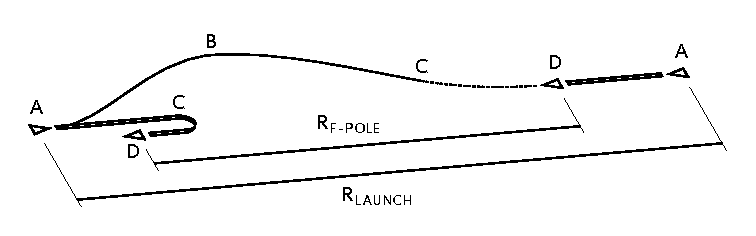
\includegraphics[
%             width = 128mm,
%     ]{F16_aaweapons_amraam_employment_v07.pdf}
%     \caption{Generic, simplified AIM-120 employment profile}
%     \label{fig:aaweap:bvr:aim120profile}
% \end{figure}

\begin{figure}[htbp]
    \centering
    \begin{tikzpicture}[auto, node distance=10mm, x=1mm, y=1mm, very thick, line cap=round,
        >={Latex[round]}
        ]
        % help lines
        % \draw[help lines] (0,-10) grid (100,10);

        % MISSILE
        \coordinate (A_missile) at (0,0);
        \coordinate (B_missile) at (30,10);
        \coordinate (C_missile) at (60,3);
        \coordinate (D_missile) at (80,0);

        \draw[thick, ->]
        (A_missile) .. controls ($(A_missile)+(20,0)$) and ($(B_missile)+(-10,0)$) .. 
        (B_missile) .. controls ($(B_missile)+(5,0)$) and ($(C_missile)+(-10,2.5)$) ..
        (C_missile);
        \draw[dotted, thick, ->] 
        (C_missile) .. controls ($(C_missile)+(10,-2.5)$) and ($(D_missile)+(-5,0)$) ..
        (D_missile);

        \node[above] at (A_missile) {\titlefont A};
        \node[above] at (B_missile) {\titlefont B};
        \node[above] at (C_missile) {\titlefont C};
        \node[above] at (D_missile) {\titlefont D};

        % FIGHTER
        \coordinate (A_fighter) at (A_missile);
        \coordinate (C_fighter) at ($(A_fighter)+(20,0)$);
        \coordinate (D_fighter) at ($(C_fighter)+(-5,-5)$);

        \draw[ultra thick, ->] 
        (A_fighter) -- 
        (C_fighter) .. controls ($(C_fighter)+(5,0)$) and ($(C_fighter)+(5,-5)$) .. 
        ($(C_fighter)+(0,-5)$) --
        (D_fighter);

        \node[above right] at (C_fighter) {\titlefont C};
        \node[left] at (D_fighter) {\titlefont D};

        % BANDIT
        \coordinate (A_bandit) at (100,0);
        \coordinate (C_bandit) at (85,0);
        \coordinate (D_bandit) at (D_missile);

        \draw[ultra thick, ->] 
        (A_bandit) -- 
        (D_bandit);

        \node[above] at (A_bandit) {\titlefont A};
        \node[above] at (C_bandit) {\titlefont C};

        \filldraw[red] (D_bandit) circle (2pt);

        % Distance lines
        \draw[thin, <->]
        ($(C_fighter)+(0,-12.5)$) -- node[pos=0.5, above]{\small\titlefont R\textsubscript{A-POLE}}
        ($(C_bandit)+(0,-12.5)$);
        \draw[thin, <->]
        (15,-20) -- node[pos=0.5, above]{\small\titlefont R\textsubscript{F-POLE}}
        ($(D_missile)+(0,-20)$);
        \draw[thin, <->]
        ($(A_missile)+(0,-27.5)$) -- node[pos=0.5, above]{\small\titlefont R\textsubscript{LAUNCH}}
        ($(A_bandit)+(0,-27.5)$);

        \draw[thin]
        ($(C_fighter)+(0,-2.5)$) -- ($(C_fighter)+(0,-15)$)
        ($(C_bandit)+(0,-2.5)$) -- ($(C_bandit)+(0,-15)$)
        ($(D_fighter)+(0,-2.5)$) -- (15,-22.5)
        ($(D_missile)+(0,-2.5)$) -- ($(D_missile)+(0,-22.5)$)
        ($(A_missile)+(0,-2.5)$) -- ($(A_missile)+(0,-30)$)
        ($(A_bandit)+(0,-2.5)$) -- ($(A_bandit)+(0,-30)$);

    \end{tikzpicture}
    \caption{Side-on view of a generic AIM-120 employment profile}
    \label{fig:aaweap:bvr:aim120profile}
\end{figure}

\begin{tcoloritemize}
    \blueitem{AIM-120 \break Employment \break Profile}{
    \Cref{fig:aaweap:bvr:aim120profile} shows the trajectories of fighter, bandit \& missile for a generic AIM-120 employment profile
    including the following phases

    \begin{subitemize}
        \item \textbf{A --- Launch / Boost Phase}
        \item \textbf{B --- Mid-Course Phase}
        \item \textbf{C --- Acquisition}
        \item \textbf{D --- Intercept}
    \end{subitemize}}
    \blueitem{Launch / Boost Phase}{
    \textbf{Boost}

    \begin{subitemize}
        \item Motor only fires for initial seconds of flight 
        \item After burnout missile \underline{cannot gain energy}
    \end{subitemize}

    \textbf{Lofting} 

    \begin{subitemize}
        \item To reach longer ranges missile ``lofts'' itself to conserve energy \& optimize trajectory
        \item Pilot can manually loft by raising the nose 20-30 deg prior to launch
    \end{subitemize}
    }
    \blueitem{Mid-Course Phase}{
    \textbf{Missile flies using internal IMU}

    \begin{subitemize}
        \item Receives periodic datalink updates
        \item Will fly to last updated target position if DL lost
    \end{subitemize}}
    \blueitem{Acquisition \& MPRF ``Active'' Phase}{
    \textbf{Missile radar turns on once close to target location}
    \begin{subitemize}
        \item Seeker in MPRF (Medium Pulse Repetition Frequency) mode 
        \item Locks on to closest / best target
    \end{subitemize}}
    \blueitem{Terminal Phase \& Intercept}{
    \textbf{Once missile seeker has acquired target}
    \begin{subitemize}
        \item Flies PNG intercept trajectory
        \item Requires no further DL support, fighter can turn away from the bandit
    \end{subitemize}}
\end{tcoloritemize}

\warningbox{
    \textbf{AIM-120 HAS \underline{NO} IFF FUNCTIONALITY} --- use caution near friendlies
}

\subsubsection{TACTICAL CONSIDERATIONS}
\label{subsec:bvr:tacticalconsideration}
% \label{subsec:aim120:tactics}
\begin{tcoloritemize}
    \blueitem{Range Definitions}{
    \textbf{Fighter-bandit distance} can be measured at different points during the timeline

    \begin{subitemize}
        \item \textbf{R\textsubscript{Launch}} --- distance at launch
        \item \textbf{R\textsubscript{A-Pole}} --- distance when missile goes active
        \item \textbf{R\textsubscript{F-Pole}} --- distance at impact
    \end{subitemize}
    
    These are also illustrated in \cref{fig:aaweap:bvr:aim120profile}.
    }
    \blueitem{Maximizing Launch Range / Energy}{
    \textbf{Why?}
    \begin{subitemize}
        \item Ability to launch at longer ranges forces bandit defensive
        \item Bandit may not be able to counter-launch
        \item Higher launch energy increases P\textsubscript{intercept} %probability of intercept
    \end{subitemize}
    \textbf{How?}
    \begin{subitemize}
        \item \textbf{High velocity} --- increases kinetic energy 
        \item \textbf{High altitude} --- increases potential energy, reduces drag
    \end{subitemize}}
    \blueitem{Maximizing \break F-Pole Range}{
    \textbf{Why?}
    \begin{subitemize}
        \item Less likely to enter bandit launch envelope
        \item More time/range to launch 2nd missile if necessary
    \end{subitemize}
    \textbf{How?}
    \begin{subitemize}
        \item \textbf{Crank} --- turn 45-60 degrees away from bandit to reduce closure rate, maintain radar contact
        \item \textbf{Dive} --- reduces threat missile envelope
    \end{subitemize}}
    \blueitem{Flowing Cold}{
    \textbf{Why?}
    \begin{subitemize}
        \item Missile requires no support once active
        \item Defend against unknown missile launches
        \item Maximize F-pole range further
    \end{subitemize}
    \textbf{How?}
    \begin{subitemize}
        \item \textbf{Turn} --- Away from bandit / threat
        \item \textbf{Dive} --- if necessary, reduces threat missile envelope 
    \end{subitemize}}
    \blueitem{Effect of Bandit Maneuvers}{
    As evident in \cref{fig:aaweap:bvr:aim120profile}, 
   \textbf{R\textsubscript{Launch}} is significantly greater than the distance travelled by the missile
    \begin{subitemize}
        \item \textbf{DLZ calculated based off \underline{both} fighter \underline{and} bandit velocity/altitude}
        \item Bandit can significantly change missile envelope by reducing closure rate / altitude
        \item Post-launch bandit maneuvers can result in missile not having energy to intercept
    \end{subitemize}}
\end{tcoloritemize}

\clearpage

\subsubsection{FIGHTER MANEUVERS}

\begin{tcoloritemize}
    \blueitem{Crank}{Fighter turns \textbf{45-60 deg} away from threat 

    \begin{subitemize}
        \item reduces closure while maintaining radar track
        \item typically used post-launch
    \end{subitemize}
    
    Reference \cref{fig:aaweap:bvr:fightermaneuver:crank}
    }
    \blueitem{Notch}{Fighter turns \textbf{70-110 deg} away from threat

    \begin{subitemize}
        \item minimizes relative velocity to break hostile pulse-doppler radar track
        \item increases angular motion, forcing missile to maneuver and expend energy
    \end{subitemize}
    
    Reference \cref{fig:aaweap:bvr:fightermaneuver:notch}
    }
    \blueitem{Go Cold}{Fighter turns \textbf{away} from threat

    \begin{subitemize}
        \item used to kinematically defeat threat missiles
    \end{subitemize}
    
    Reference \cref{fig:aaweap:bvr:fightermaneuver:cold}}
\end{tcoloritemize}

\begin{figure}[htbp]
    \centering
    \begin{subfigure}[b]{0.3\linewidth}
        \centering
        \begin{tikzpicture}[auto, node distance=10mm, x=1mm, y=1mm, very thick, line cap=round,
            >={Latex[round]}
            ]
            % FIGHTER
            \draw[ultra thick, rounded corners, ->] 
            (0,0) -- (0,5) -- +(30:15);
    
            % BANDIT
            \draw[ultra thick, rounded corners, ->] 
            (0,35) -- (0,25);
    
            % help line
            \draw[thin, dashed] 
            (0,25) -- (0,5);
    
            \draw[thin]
            (0,15) arc (90:30:10) node[pos=0.25, above right]{\small\titlefont 45-60$^\circ$};
    
        \end{tikzpicture}
        \caption{Crank}
        \label{fig:aaweap:bvr:fightermaneuver:crank}
    \end{subfigure}
    \begin{subfigure}[b]{0.3\linewidth}
        \centering
        \begin{tikzpicture}[auto, node distance=10mm, x=1mm, y=1mm, very thick, line cap=round,
            >={Latex[round]}
            ]
            % FIGHTER
            \draw[ultra thick, rounded corners, ->] 
            (0,0) -- (0,5) -- +(0:15);
    
            % BANDIT
            \draw[ultra thick, rounded corners, ->] 
            (0,35) -- (0,25);
    
            % help line
            \draw[thin, dashed] 
            (0,25) -- (0,5);
    
            \draw[thin]
            (0,15) arc (90:0:10) node[pos=0.5, above right]{\small\titlefont 70-110$^\circ$};
    
        \end{tikzpicture}
        \caption{Notch}
        \label{fig:aaweap:bvr:fightermaneuver:notch}
    \end{subfigure}
    \begin{subfigure}[b]{0.3\linewidth}
        \centering
        \begin{tikzpicture}[auto, node distance=10mm, x=1mm, y=1mm, very thick, line cap=round,
            >={Latex[round]}
            ]
            % FIGHTER
            \draw[ultra thick, ->] 
            (0,0) -- 
            (0,5) arc (180:0:5) --
            (10,0);
    
            % BANDIT
            \draw[ultra thick, rounded corners, ->] 
            (0,35) -- (0,25);

            % help line
            \draw[thin, dashed] 
            (0,25) -- (0,5);

        \end{tikzpicture}
        \caption{Go Cold}
        \label{fig:aaweap:bvr:fightermaneuver:cold}
    \end{subfigure}
    \caption{Top-down view of basic BVR fighter maneuvers}
    \label{fig:aaweap:bvr:fightermaneuver}
\end{figure}

\warningbox{
    \textbf{Turning back in after going cold can place fighter within bandit launch envelope}
}

\clearpage

\subsubsection{TARGET ASPECT}

\begin{tcoloritemize}
    \blueitem{Target Aspect}{Angle between imaginary line connecting fighter-bandit and bandit heading}
    \blueitem{Hot}{\textbf{Target aspect --- 0-40 deg}
    \begin{subitemize}
        \item offensive posture, maximizes closure
    \end{subitemize}}
    \blueitem{Flank}{\textbf{Target aspect --- 40-70 deg}
    \begin{subitemize}
        \item minimizes closure while maintaining radar track
    \end{subitemize} }
    \blueitem{Beam}{\textbf{Target aspect --- 70-110 deg}
    \begin{subitemize}
        \item defensive maneuver to break pulse-doppler radar track
    \end{subitemize}}
    \blueitem{Drag}{\textbf{Target aspect --- 110-180 deg}
    \begin{subitemize}
        \item defense to kinematically defeat missile
        \item often used in group tactics as ambush setup
    \end{subitemize}}
\end{tcoloritemize}

\begin{figure}[htbp]
    \centering
    \begin{subfigure}[b]{0.2\linewidth}
        \centering
        \begin{tikzpicture}[auto, node distance=10mm, x=1mm, y=1mm, very thick, line cap=round,
            >={Latex[round]}
            ]
            % FIGHTER
            \draw[ultra thick, rounded corners, ->] 
            (0,0) -- (0,15);
    
            % BANDIT
            \draw[ultra thick, rounded corners, ->] 
            (0,35) -- +(-75:15);
    
            % help line
            \draw[thin, dashed] 
            (0,35) -- (0,5);
    
            \draw[thin]
            (0,25) arc (-90:-75:10) node[pos=1.0, right]{\small\titlefont 0-40$^\circ$};

        \end{tikzpicture}
        \caption{Hot}
        \label{fig:aaweap:bvr:ta:hot}
    \end{subfigure}
    \begin{subfigure}[b]{0.2\linewidth}
        \centering
        \begin{tikzpicture}[auto, node distance=10mm, x=1mm, y=1mm, very thick, line cap=round,
            >={Latex[round]}
            ]
            % FIGHTER
            \draw[ultra thick, rounded corners, ->] 
            (0,0) -- (0,15);
    
            % BANDIT
            \draw[ultra thick, rounded corners, ->] 
            (0,35) -- +(-30:15);
    
            % help line
            \draw[thin, dashed] 
            (0,35) -- (0,5);
    
            \draw[thin]
            (0,25) arc (-90:-30:10) node[pos=0.25, below right]{\small\titlefont 40-70$^\circ$};

        \end{tikzpicture}
        \caption{Flank}
        \label{fig:aaweap:bvr:ta:flank}
    \end{subfigure}
    \begin{subfigure}[b]{0.25\linewidth}
        \centering
        \begin{tikzpicture}[auto, node distance=10mm, x=1mm, y=1mm, very thick, line cap=round,
            >={Latex[round]}
            ]
            % FIGHTER
            \draw[ultra thick, rounded corners, ->] 
            (0,0) -- (0,15);
    
            % BANDIT
            \draw[ultra thick, rounded corners, ->] 
            (0,35) -- +(0:15);
    
            % help line
            \draw[thin, dashed] 
            (0,35) -- (0,5);
    
            \draw[thin]
            (0,25) arc (-90:0:10) node[pos=0.25, below right]{\small\titlefont 70-110$^\circ$};
    
        \end{tikzpicture}
        \caption{Beam}
        \label{fig:aaweap:bvr:ta:beam}
    \end{subfigure}
    \begin{subfigure}[b]{0.25\linewidth}
        \centering
        \begin{tikzpicture}[auto, node distance=10mm, x=1mm, y=1mm, very thick, line cap=round,
            >={Latex[round]}
            ]
            % FIGHTER
            \draw[ultra thick, rounded corners, ->] 
            (0,0) -- (0,15);
    
            % BANDIT
            \draw[ultra thick, rounded corners, ->] 
            (0,35) -- +(90:15);
    
            % help line
            \draw[thin, dashed] 
            (0,35) -- (0,5);
    
            \draw[thin]
            (0,25) arc (-90:90:10) node[pos=0.125, below right]{\small\titlefont 110-180$^\circ$};
    
        \end{tikzpicture}
        \caption{Drag}
        \label{fig:aaweap:bvr:ta:drag}
    \end{subfigure}
    \caption{Top down view illustrating target aspect terminology}
    \label{fig:aaweap:bvr:ta}
\end{figure}

\marginfigeometry

\subsubsection{BVR TIMELINE --- WIP}

\marginfigrestore